\chapter{AlgTest pyProcess tool}
This chapter describes the development details behind the tool called \texttt{AlgTest pyProcess}, creation of which was main goal of this thesis. Its development began as a reimplementation of tool called \texttt{JCAlgTest Process}. The reasons behind the reimplementation are mentioned in previous chapter.

The \texttt{AlgTest pyProcess} tool responsible for the following tasks:
\begin{itemize}
    \item Processing the device profiles generated by automatic testing tools targeted at Trusted Platform Modules and JavaCard smart cards,
    \item Generation of various outputs from these datasets which are primarily tabular and graphical visualizations.
\end{itemize}
\begin{figure}[h]
    \centering
    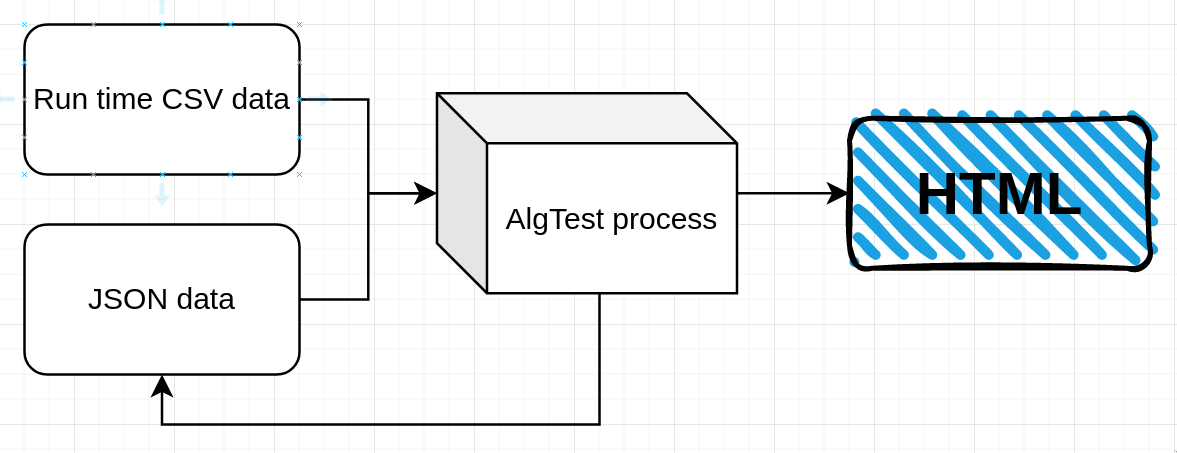
\includegraphics[width=\textwidth]{img/scheme.png}
    \caption{Scheme of AlgTest pyProcess application}
    \label{fig:algtest-process-scheme}
\end{figure}


\section{Parsing}
The \texttt{AlgTest pyProcess} tool is working with datasets that were generated and collected over the years in parallel with the development of the testing tools which generate these datasets. The outputs of these testing tools have been changing over the years too, that is why the testing form of output format for tested devices may differ depending on the version of the testing tool.

There is no prescribed schema for the datasets, but they generally look very similar\footnote{Examples of CSV device profiles are shown in Appendix}. That is why it is convenient to design suitable means of accessing the data contained in them. Such means are provided by mapping these profiles onto class representation. But first step in order to accomplish that is the parsing the CSV files which represent the device profiles. 



\section{Results}
The tool produces various visualization and tables as HTML files, which any modern web browser can view. The contents are made responsive and interactive and try to provide convenient means of getting information about the select devices compared to other devices. 

These visualizations may be helpful for various types of audiences:

\begin{itemize}
    \item \texttt{Potential buyers} who want to select their device which suits their needs for supported algorithms or just want to get some insight about the ecosystem, such as what vendors are available. 
    
    \item \texttt{The developers} of software for these devices who want to get the knowledge of the device they are supposed to develop applications for. Insight into the supported algorithms and their performance may enable them to make tailor-made adjustments that may improve the developed application's performance and functionality.
\end{itemize}

The \myref{Table}{table:results} shows the available visualisations for both TPMs and JavaCard smart cards. In the following sections each result will be presented separately.

\begin{table}[H]
    \begin{adjustbox}{max width=\textwidth}
    \begin{tabular}{c|c|c|c|c|c|c|c}
         Device     & Support & Similarity & Execution time & Radar  & Heatmap   & Comparative & Scalability \\ \hline
         TPM        & \cmark  & \cmark     & \cmark         & \cmark & \cmark    & \xmark      & \xmark  \\ \hline
         JavaCard   & \cmark  & \cmark     & \cmark         & \cmark & \xmark    & \cmark      & \cmark  
    \end{tabular}
    \end{adjustbox}
    \caption{Results generated for each device}
    \label{table:results}
\end{table}

\subsection{Support table}
The support table contains information about support for a particular algorithm from the specific smart card. During the test for algorithm support, we can get multiple results. Either the algorithm is supported,  unsupported, error was returned, or lastly, the algorithm was not tested. Each of these results is denoted by the content and the color of the cell. By hovering over the error cell, we can find out what kind of exception or error was returned from the card. The table also provides means to filter the cards according to their support for categories of algorithms.

\begin{figure}[H]
    \centering
    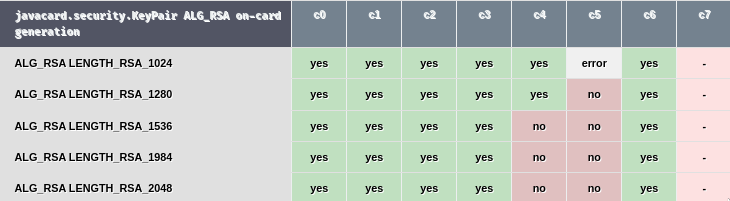
\includegraphics[width=\textwidth]{img/support-table.png}
    \caption{Support table}
    \label{fig:support-table}
\end{figure}

\subsection{Similarity table}
The similarity table shows how a chosen pair of cards differ in the performance of a selected group of operations. The similarity is computed for six different categories of algorithms and results in a percentage on a scale of 0 to 100, also signified by the color of each cell. The higher number indicates higher performance similarity. The cards in the table are sorted so that most similar cards are in the top left corner and the least similar are in the bottom right corner.

\begin{figure}[H]
    \centering
    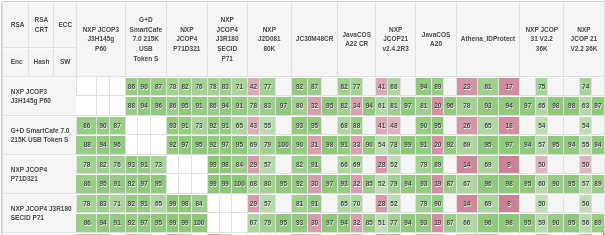
\includegraphics[width=\textwidth]{img/similarity-table.png}
    \caption{Similarity table}
    \label{fig:similarity-table}
\end{figure}

\subsection{Algorithm execution time}
Algorithm execution time pages are generated for each card separately and present an alternative for searching in the corresponding raw CSV file. The page contains metadata detailing the test performed on this smart card, followed by tables containing algorithm measurement values. There are multiple tables because the tested algorithms are divided into numerous categories. A quick link for each of these categories is provided as a utility to aid searching on the page.

\begin{figure}[H]
    \centering
    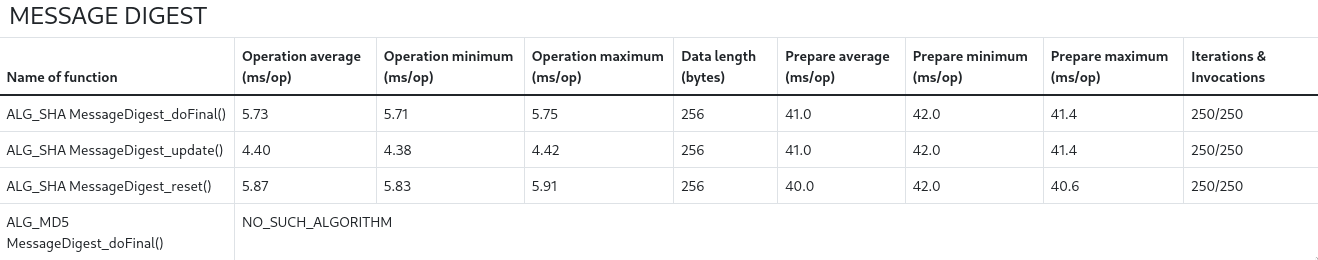
\includegraphics[width=\textwidth]{img/NXP JCOP4 P71D321 execution-time table.png}
    \caption{Algorithm execution timetable of NXP JCOP4 P71D321}
    \label{fig:execution-time-table}
\end{figure}

\subsection{Radar graphs}
Radar graphs visualize the card's performance compared to all other tested cards. A percentage describes overall performance on a scale of 0 to 100, where closer to 100 is faster. Zero value signifies either that the algorithm is not supported or not successfully tested. By hovering over the points on edge, we can see the actual average operation time for the chosen algorithm. The algorithms chosen for comparison were selected as most frequently used, and in the context of the tool, we call them Top Functions. 

\begin{figure}[H]
    \centering
    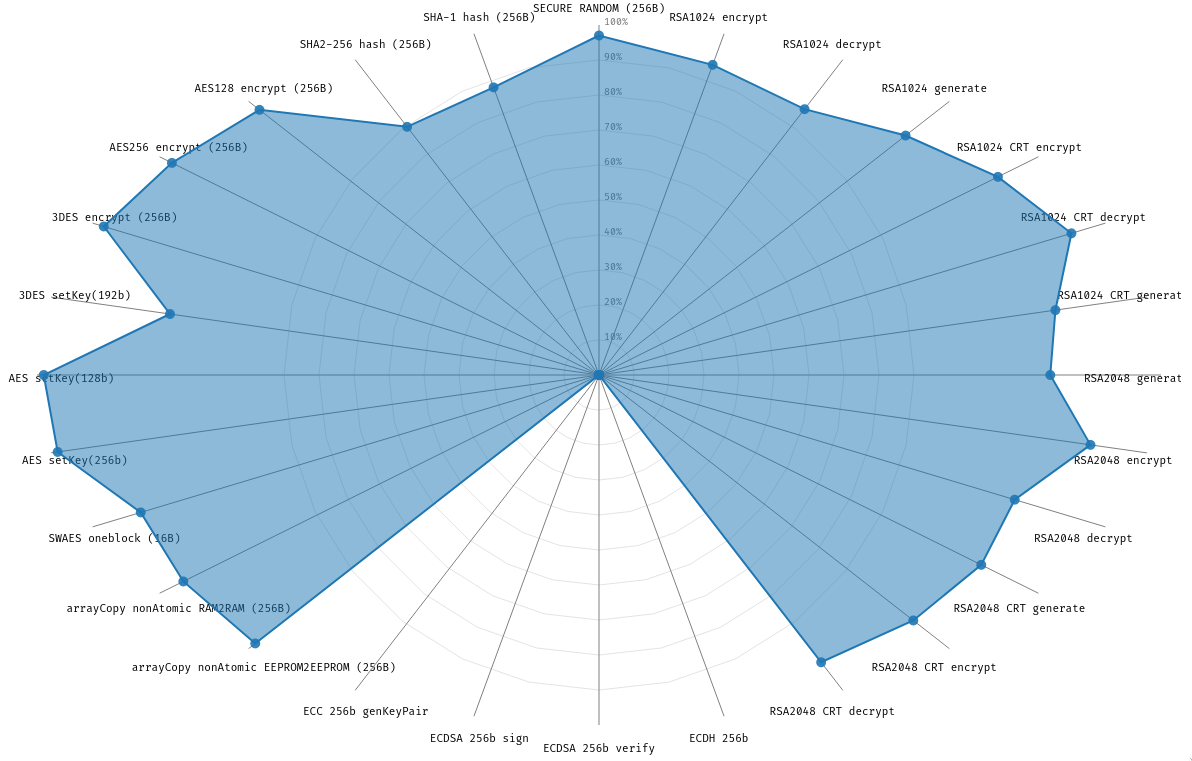
\includegraphics[width=\textwidth]{img/JC30M48CR radar graph.png}
    \caption{
    The radar graph of the JC30M48CR card  can be considered excellent, apart from no evident support for algorithms involving Elliptic Curve Cryptography signified by a cut-out at the bottom of the graph.
    }
    \label{fig:radar-graph}
\end{figure}

\subsection{Comparative table}
The comparative table allows for a simple comparison between cards. Multiple comparative tables are generated in one file divided into symmetric, asymmetric cryptography, and frequently used algorithms, also called Top Functions. The tables themselves allow for sorting of the cards just by simply clicking on the column containing values according to which rows will be sorted.

\begin{figure}[H]
    \centering
    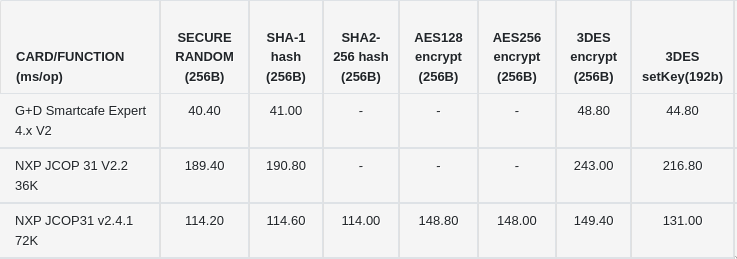
\includegraphics[width=\textwidth]{img/comparative-table.png}
    \caption{Comparative table}
    \label{fig:comparative-table}
\end{figure}

\subsection{Scalability graphs}
Scalability graphs illustrate a single card's performance for a specific algorithm depending on input data length. The graph is generated for each method that was measured. The time scale from minimum to maximum measurement value for each measurement of the given algorithm and average time both in milliseconds can be found by simply hovering over the point in the graph.

\begin{figure}[H]
    \centering  
    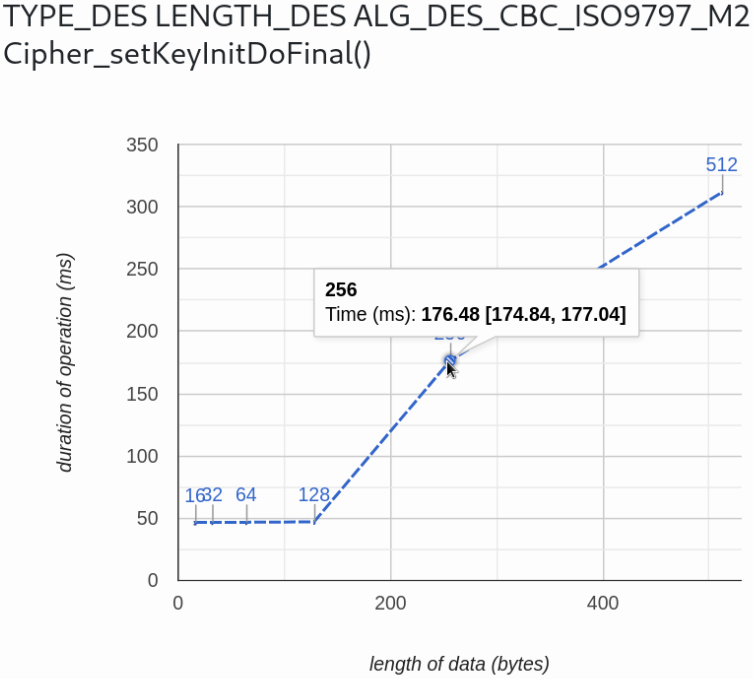
\includegraphics[width=\textwidth-3.5cm]{img/NXP_JCOP_J3D081_v2.4.2R2 scalability graph.png}
    \caption{
    Scalability chart of NXP JCOP J3D081 v2.4.2R2 showing performance of DES algorithm in CBC mode, for data lengths We can observe 16, 32, 64, 128 bits the performance seems to be constant, following 256, 512 bits an almost linear increase.
    }
    \label{fig:scalability-chart}
\end{figure}




\section{Tools}
The \texttt{AlgTest process} tool incorporates various instruments to produce desired outputs. As the tool itself is written in Python it is able to utilize various packages from \texttt{PyPI}\footnote{\url{https://pypi.org/}} to aid future extensions.

\begin{itemize}
    \item For creation and manipulation of HTML documents a Python library called \texttt{dominate}\footnote{\url{https://pypi.org/project/dominate/}} is used. Its usage is relatively straightforward, and the code you write is in pure python instead of using additional templating language as in popular web frameworks.
    \item The styling is taken care of by a CSS framework called \texttt{bootstrap}\footnote{\url{https://getbootstrap.com/}} which allows for designing responsive web pages using premade CSS classes and Javascript. The framework itself is extensively used and regularly updated with new versions.
    \item \texttt{Google Charts API}\footnote{\url{https://developers.google.com/chart}}  is utilized for Scalability graph visualisation.
    \item \texttt{D3.js library}\footnote{\url{https://d3js.org/}}  is used for visualisation of Radar graphs.
\end{itemize}

